\section{Results}
\label{sec:results}

We first establish baselines and the noise floor (\secref{sec:baselines}). We then test H1 on edit types (\secref{sec:h1}), H2 on task types (\secref{sec:h2}) and H3 on compounding (\secref{sec:h3}), and finally relate fragility to edit size (\secref{sec:magnitude}).

\subsection{Baselines and noise floor}
\label{sec:baselines}

\begin{table}[t]
\centering
\small
\begin{tabular}{@{}lcccc@{}}
\toprule
 & \sst & \agnews & \arc & \squad (F1) \\
\midrule
\qwen, original prompt & {\bf 93.0} & {\bf 75.0} & {\bf 72.0} & {\bf 88.5} \\
\llama, original prompt & 75.0 & 25.0$^\dagger$ & 49.0 & 71.6 \\
\midrule
\qwen, rerun of original: flip rate & 2\% & 0\% & 1\% & 0\% \\
\llama, rerun of original: flip rate & 1\% & 0\% & 0\% & 0\% \\
\bottomrule
\end{tabular}
\caption{Scores with the original prompt and the noise floor. The bottom rows show the share of items whose correctness changes when the identical prompt is resubmitted. Changes of 2 points or less are within noise. $^\dagger$\llama predicts ``World'', the first label listed, for 98 of 100 \agnews items, so this cell is at chance. Best score per task in \textbf{bold}.}
\label{tab:baselines}
\end{table}

\Tabref{tab:baselines} shows the original-prompt scores. \qwen is the stronger model on every task. llama.cpp's continuous batching is slightly nondeterministic: resubmitting the identical prompt changes correctness on 0--2\% of items. We therefore treat effects of 2 points or less as noise. \llama is degenerate on \agnews: it answers ``World'', the first label listed in the instruction, for 98\% of items. A relative index is meaningless at a chance-level baseline, so we report this cell but exclude it from pooled conclusions. We made this exclusion after seeing the baseline.

\subsection{H1: no edit type is uniformly harmful or harmless}
\label{sec:h1}

\begin{table}[t]
\centering
\resizebox{\textwidth}{!}{%
\begin{tabular}{@{}lcccccccc@{}}
\toprule
 & \multicolumn{4}{c}{\qwen} & \multicolumn{4}{c}{\llama} \\
\cmidrule(lr){2-5} \cmidrule(lr){6-9}
\textbf{Edit} & \sst & \agnews & \arc & \squad & \sst & \agnews$^\dagger$ & \arc & \squad \\
\midrule
\ws    & $-$1.5 \ci{$-$5.0}{1.0} & 0.5 \ci{$-$3.5}{4.0} & 3.0 \ci{$-$1.0}{7.0} & 2.6 \ci{0.6}{5.0} & $-$0.5 \ci{$-$3.5}{2.5} & $-$6.0 \ci{$-$11.5}{$-$0.5} & $-$1.0 \ci{$-$3.5}{1.5} & 1.5 \ci{$-$2.6}{5.5} \\
\caps  & 0.5 \ci{$-$3.0}{4.0} & {\bf 25.0}* \ci{17.0}{33.5} & 2.5 \ci{$-$1.0}{7.0} & 2.4 \ci{0.3}{4.7} & 6.0 \ci{2.0}{10.0} & 0.0 & $-$0.5 \ci{$-$5.0}{4.0} & 2.9 \ci{$-$0.5}{6.3} \\
\punct & 0.0 \ci{$-$2.0}{2.0} & {\bf 16.0}* \ci{10.0}{22.0} & 2.0 \ci{$-$2.0}{6.5} & 5.2 \ci{1.7}{8.7} & $-$2.5 \ci{$-$6.5}{1.5} & 0.0 & 10.5 \ci{3.5}{17.5} & 0.8 \ci{$-$0.8}{2.4} \\
\typo  & 0.5 \ci{$-$3.0}{3.5} & $-$1.0 \ci{$-$4.5}{1.5} & 2.0 \ci{$-$2.5}{7.0} & 1.2 \ci{$-$1.5}{4.0} & $-$2.5 \ci{$-$7.0}{1.5} & 0.0 & 0.5 \ci{$-$5.0}{6.0} & $-$1.8 \ci{$-$5.4}{1.6} \\
\syn   & 0.0 \ci{$-$3.0}{2.5} & 2.5 \ci{$-$4.0}{8.5} & 4.0 \ci{0.0}{8.5} & 2.1 \ci{$-$1.2}{5.5} & $-$6.0 \ci{$-$11.5}{$-$1.0} & $-$6.5 \ci{$-$12.0}{$-$0.5} & {\bf 14.5}* \ci{8.5}{20.5} & 0.2 \ci{$-$4.6}{4.9} \\
\reord & 1.0 \ci{$-$3.0}{5.0} & 4.0 \ci{0.5}{7.5} & 3.5 \ci{$-$0.5}{8.0} & 2.7 \ci{0.5}{5.2} & $-$7.0* \ci{$-$12.0}{$-$2.5} & $-$11.0* \ci{$-$17.0}{$-$5.5} & 4.5 \ci{$-$0.5}{10.0} & $-$2.8 \ci{$-$6.6}{0.6} \\
\bottomrule
\end{tabular}%
}
\caption{Score drop $\Delta$ (points; positive means the edit hurts) for each single edit type, averaged over 2 seeds, with paired 95\% bootstrap CIs. * marks Holm-adjusted $p<0.05$. Drops above the 8-point threshold of H1 that are also significant are in \textbf{bold}. $^\dagger$Degenerate baseline (\tabref{tab:baselines}). The damaging edit differs by model and task: \caps and \punct break \qwen on \agnews only, \syn breaks \llama on \arc only, and \reord significantly \emph{helps} \llama on \sst and \agnews.}
\label{tab:h1}
\end{table}

\begin{figure}[t]
\centering
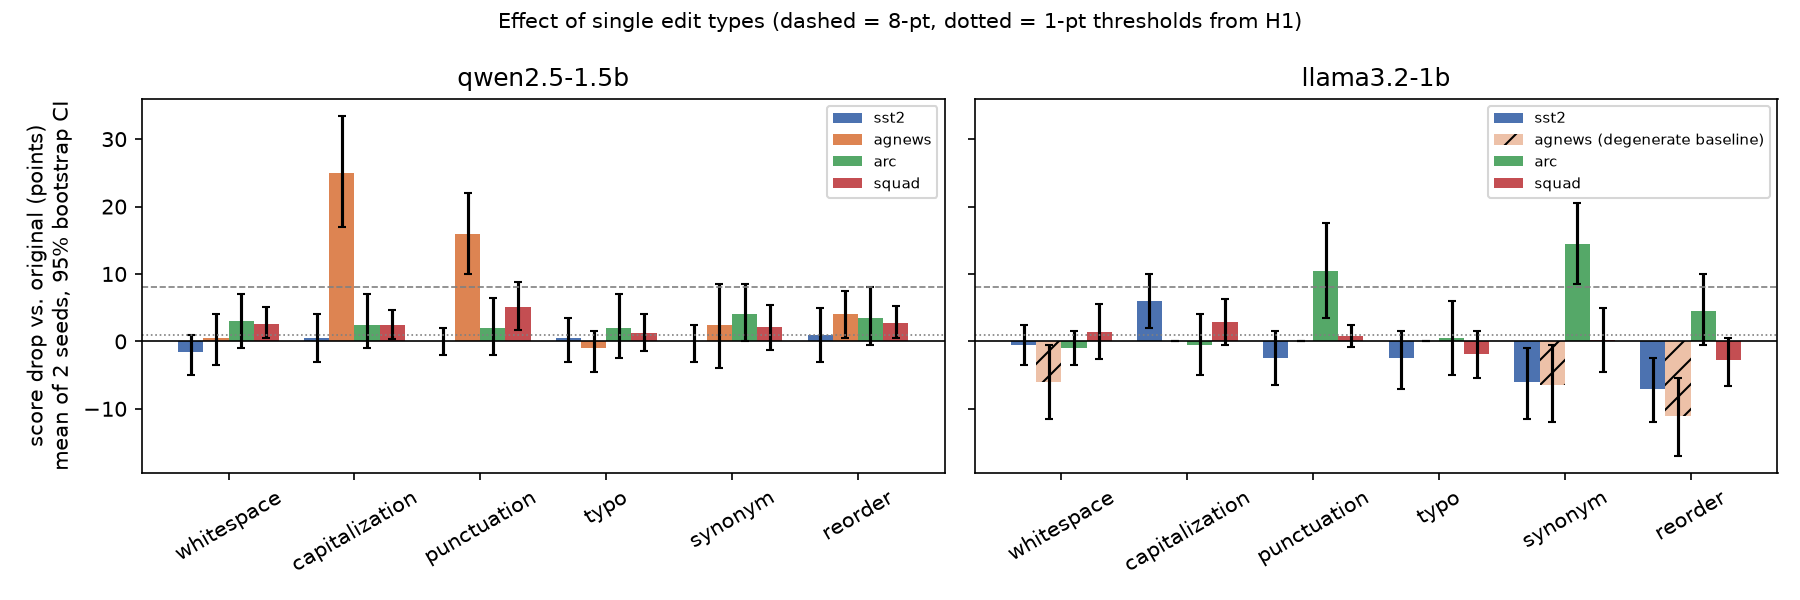
\includegraphics[width=0.95\linewidth]{figures/edit_type_by_model.png}
\caption{Score drop for each single edit type, by task, for \qwen \figleft and \llama \figright (mean of 2 seeds; error bars are 95\% bootstrap CIs). The dashed and dotted lines mark H1's 8-point and 1-point thresholds. Only three cells are significant drops above 8 points, and none of them belongs to \reord. Negative bars are edits that \emph{improve} the score.}
\label{fig:h1}
\end{figure}

\Tabref{tab:h1} and \figref{fig:h1} report the drop caused by each single edit type, and \tabref{tab:h1_pooled} pools these drops over tasks. H1 predicted that \reord and \syn would cost more than 8 points while \ws and \caps would cost less than 1 point. The data refute both halves.

{\bf Which edits hurt?} The largest drops come from edits that H1 called harmless. For \qwen on \agnews, \caps costs 25.0 points (CI [17.0, 33.5]) and \punct costs 16.0 points (CI [10.0, 22.0]). Both survive Holm correction. The same two edits cost \qwen at most 0.5 points on \sst. For \llama, the largest drops are \syn on \arc (14.5 points) and \punct on \arc (10.5 points, not significant after correction). \Secref{sec:mechanisms} shows that the first is mostly a format effect and the second a content effect.

{\bf Which edits are safe?} \reord never costs more than 4.5 points on any valid task. It significantly \emph{improves} \llama on \sst (by 7.0 points) and on \agnews (by 11.0 points). \syn never costs \qwen more than 4.0 points. \typo is the most benign edit overall (at most 2.0 points). \ws is the only edit type whose effect is small on every valid task ($|\Delta| \leq 3$ points), although its \squad CI for \qwen lies just above the 1-point threshold.

{\bf Net drops understate churn.} The flip rate of an edit type ranges from 2--8\% in robust cells to 32\% for \qwen \agnews under \caps and 25.5\% for \llama \arc under \punct. Flip rates are often several times larger than the net $|\Delta|$, because the same edit fixes some items while breaking others (\figref{fig:flip} in \appref{app:figures}).

\begin{table}[t]
\centering
\small
\begin{tabular}{@{}lccp{0.34\linewidth}@{}}
\toprule
\textbf{Edit} & \qwen & \llama\ {\scriptsize(excl.\ \agnews)} & \textbf{Verdict on H1} \\
\midrule
\ws    & 1.2 (3.0)  & 0.0 (1.5)  & \textit{roughly supported} (small everywhere) \\
\caps  & {\bf 7.6} (25.0) & 2.8 (6.0) & \textit{refuted} (not below 1 point) \\
\punct & 5.8 (16.0) & 2.9 (10.5) & not in H1; large on some tasks \\
\typo  & 0.7 (2.0)  & $-$1.3 (0.5) & not in H1; robust \\
\syn   & 2.1 (4.0)  & 2.9 (14.5) & \textit{refuted} for \qwen; above 8 only for \llama on \arc (a format effect) \\
\reord & 2.8 (4.0)  & $-$1.8 (4.5) & \textit{refuted} (never above 8 points) \\
\bottomrule
\end{tabular}
\caption{Mean drop (points) over valid tasks, with the largest single-task drop in parentheses. The largest mean drop is in \textbf{bold}.}
\label{tab:h1_pooled}
\end{table}

\subsection{H2: generation is not the most fragile task type}
\label{sec:h2}

\begin{table}[t]
\centering
\small
\begin{tabular}{@{}llcc@{}}
\toprule
\textbf{Task} & \textbf{Type} & \qwen & \llama \\
\midrule
\sst    & classification  & 0.001 \ci{$-$0.03}{0.03} & $-$0.028 \ci{$-$0.07}{0.02} \\
\agnews & classification  & {\bf 0.104} \ci{0.06}{0.15} & (degenerate) \\
\arc    & multiple choice & 0.039 \ci{$-$0.01}{0.09} & {\bf 0.097} \ci{0.02}{0.18} \\
\squad  & generation      & 0.031 \ci{0.01}{0.05} & 0.002 \ci{$-$0.04}{0.04} \\
\midrule
\multicolumn{2}{@{}l}{Classification mean (H2 predicted 0.05)} & 0.053 & $-$0.028 \\
\multicolumn{2}{@{}l}{Generation (H2 predicted 0.22)} & 0.031 & 0.002 \\
\bottomrule
\end{tabular}
\caption{Mean \pfi over the 12 single-edit conditions of each task, with item-bootstrap 95\% CIs. The most fragile task for each model is in \textbf{bold}. Generation is far below the predicted 0.22 for both models.}
\label{tab:h2}
\end{table}

\begin{figure}[t]
\centering
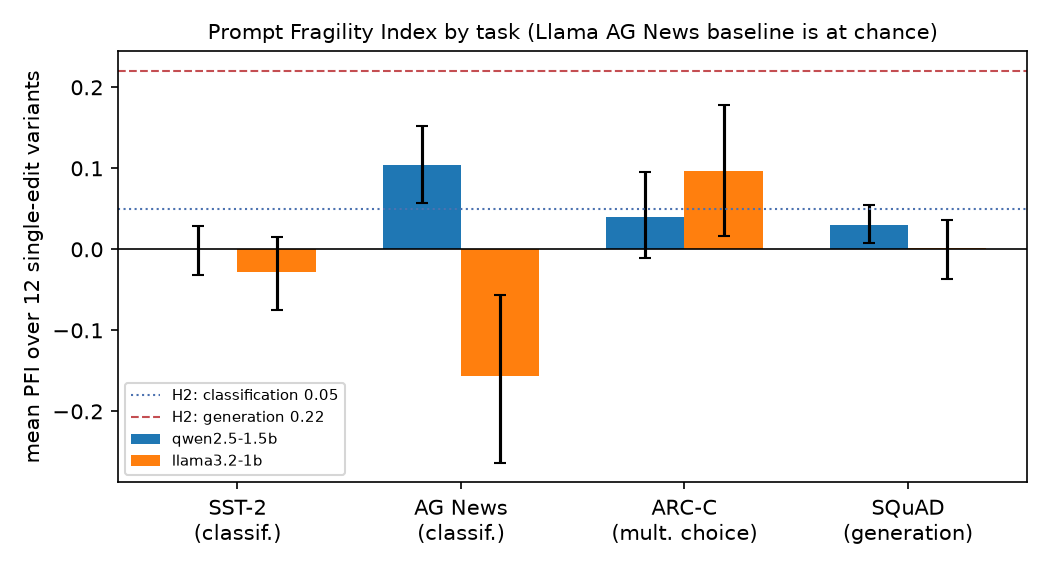
\includegraphics[width=0.62\linewidth]{figures/pfi_by_task_model.png}
\caption{Mean \pfi over the 12 single-edit conditions, by task and model, with 95\% bootstrap CIs. The dotted and dashed lines show the values H2 predicted for classification (0.05) and generation (0.22). The negative \llama \agnews bar comes from its chance-level baseline (edits break its first-label collapse) and is not a real robustness gain.}
\label{fig:h2}
\end{figure}

H2 predicted that classification would be the most robust task type (mean \pfi about 0.05) and generation the most fragile (about 0.22). \Tabref{tab:h2} and \figref{fig:h2} refute this. Generation has a mean single-edit \pfi of only 0.031 for \qwen and 0.002 for \llama. The most fragile task is \agnews for \qwen (0.104) and \arc for \llama (0.097). The classification mean for \qwen (0.053) matches the predicted 0.05 only as an average of a near-zero \sst (0.001) and a fragile \agnews. The two classification tasks lie at opposite ends of the range, which shows that task type is a poor predictor of fragility. Including the combined conditions raises \qwen's \squad \pfi to 0.081 [0.05, 0.11], because of the super-additive compounding we report next, but this is still below \agnews (0.190).

\subsection{H3: edits compound super-additively only for generation}
\label{sec:h3}

\begin{table}[t]
\centering
\resizebox{\textwidth}{!}{%
\begin{tabular}{@{}llcccccc@{}}
\toprule
\textbf{Task} & $k$ & $\Delta$ combined & Additive baseline & Ratio & Interaction vs.\ additive & Union baseline & Interaction vs.\ union \\
\midrule
\sst    & 3 & 0.8  & 0.7  & ---  & $+$0.2 \ci{$-$4.7}{5.7} & 4.0 & $-$3.2 \ci{$-$6.7}{$-$0.5} \\
\agnews & 3 & 21.0 & 26.2 & 0.80 & $-$5.2 \ci{$-$12.2}{1.7} & 27.7 & $-$6.7 \ci{$-$11.0}{$-$2.3} \\
\agnews & 6 & 36.0 & 47.0 & 0.77 & $-$11.0 \ci{$-$28.5}{6.5} & 43.0 & $-$7.0 \ci{$-$14.5}{0.5} \\
\arc    & 3 & 4.2  & 9.0  & 0.46 & $-$4.8 \ci{$-$13.2}{3.2} & 7.5 & $-$3.3 \ci{$-$6.8}{$-$0.2} \\
\arc    & 6 & 6.5  & 17.0 & 0.38 & $-$10.5 \ci{$-$30.0}{8.0} & 9.5 & $-$3.0 \ci{$-$8.0}{1.5} \\
\midrule
\squad  & 2 & 7.9  & 4.9  & {\bf 1.61} & $+$3.0 \ci{0.3}{5.9} & 5.5 & $+$2.4 \ci{$-$0.4}{5.1} \\
\squad  & 3 & 11.1 & 7.8  & {\bf 1.42} & $+$3.3 \ci{$-$2.2}{8.2} & 7.7 & $+$3.3 \ci{$-$0.6}{7.2} \\
\squad  & 6 & 20.9 & 16.2 & {\bf 1.29} & $+$4.7 \ci{$-$6.5}{15.0} & 10.7 & {\bf $+$10.2} \ci{4.3}{16.3} \\
\bottomrule
\end{tabular}%
}
\caption{Compounding for \qwen, pooled over all combinations with $k$ edit types and both seeds (points). Ratio is $\Delta$(combined) divided by the sum of single-edit drops (omitted for \sst, where both are near 0). Interaction CIs come from the item bootstrap. Super-additive results are in \textbf{bold}. Combined edits are super-additive only on \squad, and only \combo{all6} clearly exceeds the union baseline.}
\label{tab:h3}
\end{table}

\begin{figure}[t]
\centering
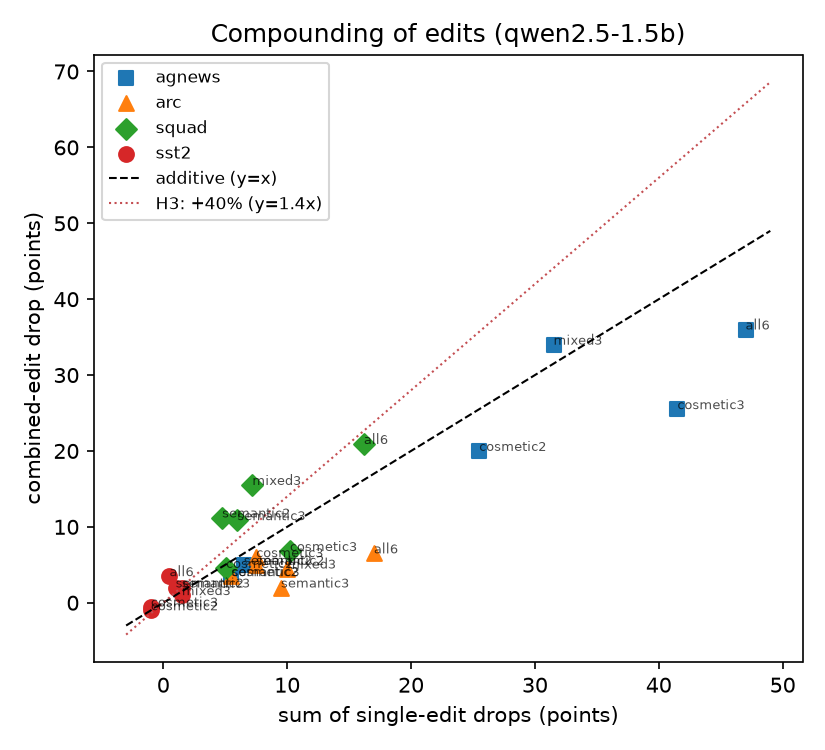
\includegraphics[width=0.5\linewidth]{figures/compounding_qwen2_5-1_5b.png}
\caption{Drop of each combined edit against the sum of the drops of its parts, for \qwen (each point is one combination at one seed). Points above the dashed line are super-additive; the dotted line is H3's $+$40\% prediction. Only \squad combinations (green) lie above the additive line. \agnews and \arc combinations lie below it, because items broken by one edit cannot break again.}
\label{fig:h3}
\end{figure}

H3 predicted that combining three or more edit types would exceed the sum of their individual effects by 30--50\%. \Tabref{tab:h3} and \figref{fig:h3} show the results for \qwen.

{\bf Generation compounds.} On \squad, combined edits exceed the additive baseline, with ratios of 1.61 for $k=2$, 1.42 for $k=3$ and 1.29 for $k=6$, close to the hypothesized range. The evidence is moderate, however. At $k=3$, the interaction CI includes 0 against both baselines. Only \combo{all6} clearly exceeds the union baseline ($+$10.2 points, CI [4.3, 16.3]).

{\bf Classification and multiple choice saturate.} On \agnews and \arc, combined edits are sub-additive, with ratios of 0.38--0.80. They break even fewer items than the union baseline predicts (for example $-$6.7 points, CI [$-$11.0, $-$2.3], for \agnews at $k=3$). The additive baseline overstates the no-interaction prediction because it counts an item broken by two edits twice. The negative union interaction means that a combination breaks fewer items than its parts do individually, which suggests that some edits partly cancel each other's damage.

{\bf \llama.} For \llama, the single-edit drops have mixed signs (for example, the sum of single drops on \sst is negative), so additive ratios are unstable. Against the union baseline, the interaction is negative in 5 of the 6 \sst and \squad cells, with all 5 CIs below 0. The exception is \sst \combo{all6} ($+$4.0, CI [$-$4.5, 12.5]). It is also negative in all three cells of the degenerate \agnews task. On \arc it is $-$3.8, $-$2.7 and $-$11.5 points for $k = 2$, 3 and 6. Individual \arc combinations can still be strongly super-additive: \combo{semantic3} at seed 0 loses 48 points against 33 for the sum of its parts, and \combo{mixed3} at seed 0 loses 40 against 26. \Secref{sec:format} traces these losses to output-format failures. Overall, H3 holds only for generation in one model.

\subsection{Larger edits cause more churn, not reliably more damage}
\label{sec:magnitude}


The character-level edit distance between the original and edited instruction correlates with the flip rate for both models (Spearman $\rho = 0.46$ for \qwen and $0.51$ for \llama, $p < 10^{-5}$, $n = 96$ conditions). It correlates with the net drop only for \qwen ($\rho = 0.44$; $\rho = 0.02$ for \llama). Larger edits change more individual answers, but whether they lower the net score depends on what they touch.
